% §3 The admissible cone --- blueprint chapter 8 (blueprint/src/parts/08-cone.tex), statements
% and proofs of record verbatim. Drafted 2026-09-15 from the blueprint at the state after
% ledger A10's admission (R162); prose rewritten 2026-09-17 at the author's review.
%
% The author's findings on the first draft (2026-09-17), and what was done:
%   - no map: the section opens with an overview of its four steps and what each buys;
%   - "the causal cone of the half-line" assumed the causal article was read: the comparison
%     is now written for a reader who has not, and the detail stays in rem:cone-shape, this
%     section's one relation-to-the-causal-theory remark (ADR-0003);
%   - two figures: fig-admissible-cone (the line paper's Figure 6 redrawn for what this paper
%     shows, TikZ) after prop:choquet-cone, and fig-cin-rays (figures/fig-cin-rays.png from
%     scripts/make-fig-cin-rays.py: the profiles, the exponents, the kernel) after lem:cin-rays;
%   - the inline prose on what is machine-checked is removed from the section body: the trust
%     base is section 1.1's, and what a proof owes to a cited fact is said inside the proof;
%   - "Choquet structure", "Levy pair", "Levy density", "delay equation", "singularity",
%     "variance-gamma" are introduced at first use, each with its citation; every subsection
%     opens with what its result says and why, and discusses the proof after the statement;
%   - the folding convention is motivated (the sources' theorems are stated two-sided; the
%     factor 2 is where a constant is lost);
%   - literature: Choquet's theorem (Phelps), the Dickman function and its delay equation
%     (Dickman 1930), the Dickman subordinator (Caravenna, Sun, Zygouras), Sato's two theorems
%     at the origin, the DLMF for Cin, Madan and Seneta for the variance-gamma laws.
%
% Contents and departures from the blueprint chapter (unchanged from the first draft):
%   - all six statement nodes transcribed under their markers: lem:cin-rays, prop:choquet-cone,
%     lem:cin-delay-equation, lem:folding-translation, prop:cin-origin-singularity (the one [A]
%     node, ledger A10, admitted 2026-09-15: its page anchors are printed in the prose before
%     the statement, read from blueprint/AXIOMS.md) and cor:origin-boundedness;
%   - lem:cin-rays is also Appendix A.1 of the line paper; it is a node of this chapter and is
%     stated here in full, with its remark;
%   - rem:cin-constant, rem:cone-shape and rem:cin-propagation are copied (remarks carry no
%     marker); rem:cone-shape names the causal article where the blueprint says "the causal
%     cone", and its first sentences now say what the causal objects are;
%   - the blueprint's status annotations are not transcribed;
%   - references to the line paper's nodes print as that paper's v0.1 numbers through the
%     \ref wrapper of macros.tex, or as the local numbers of section 2's restatements.

\section{The admissible cone: the Gaussian ray and the \texorpdfstring{$\Cin$}{Cin} rays}
\label{sec:cone}

The line paper ends with a set: the admissible exponents, the functions $F$ of the form
\ref{eq:sd-profile}, one for each admissible family in its canonical gauge. It shows that
the set is a convex cone (Lemma~\ref{lem:admissible-cone}) and stops. This section describes
the cone. The description has four steps, one subsection each. The cone is generated by one family of
simple members, the $\Cin$ rays, whose profiles are unit steps: a nonincreasing profile is a
stack of unit steps, so every admissible exponent is a Gaussian term plus a superposition of
$\Cin$ rays (\S\ref{sec:cin-rays}, Lemma~\ref{lem:cin-rays}, Figure~\ref{fig:cin-rays}). The
superposition is unique, so the Gaussian coefficient and the tail measure $\varpi = -dk$ of
the profile are coordinates on the cone, and its extreme rays are the Gaussian ray and the
$\Cin$ rays (\S\ref{sec:choquet}, Proposition~\ref{prop:choquet-cone},
Figure~\ref{fig:admissible-cone}); none of the named families of the later sections is
extreme, apart from the Gaussian endpoint of the stable family. The kernel of a ray has no
closed form and satisfies a delay equation, the twin of the equation of the Dickman function
(\S\ref{sec:delay-equation}, Lemma~\ref{lem:cin-delay-equation}). And what a kernel with
no Gaussian part does at the origin is decided by one number, the value $k(0{+})$ of its
profile there: the kernel is bounded exactly when that value exceeds $1$
(\S\ref{sec:origin}, Proposition~\ref{prop:cin-origin-singularity},
Corollary~\ref{cor:origin-boundedness}). A reader who wants the criterion alone can go to
\S\ref{sec:origin} directly, which uses the earlier subsections only for its examples.

The causal theory, on the temporal half-line, has a cone of the same shape. The comparison is
Remark~\ref{rem:cone-shape}, and nothing in this section depends on it.

\subsection{The unit-step profiles and the superposition}\label{sec:cin-rays}

The function $\Cin$ is the entire cosine integral,
$\Cin(z) = \int_0^z (1 - \cos v)\,v^{-1}dv$ (\sscite{dlmf2026}, \S6.2). The lemma first
records the two facts about it that the section uses: it starts like $z^2/4$ and grows like
$\log z$. It then gives the two facts about the unit-step profiles. Each is admissible with
$\Cin$ as its exponent, and every admissible exponent is a superposition of them.

% shared with blueprint lem:cin-rays
\begin{lemma}[the $\Cin$ rays and the superposition]\label{lem:cin-rays}
Write $\Cin(z) := \int_0^z (1 - \cos v)\,v^{-1}dv$ for $z \ge 0$, extended evenly to $\RR$.
\begin{enumerate}
\item \emph{(The rays.)} For $\tau > 0$ the profile $k = \mathbf 1_{(0,\tau)}$ is admissible,
with Gaussian coefficient $0$, and its exponent is $\omega \mapsto \Cin(\tau\omega)$. The
function $\Cin$ is even and nondecreasing on $[0,\infty)$, with $\Cin(z) \le z^2/4$ and
$\Cin(z) = \tfrac14 z^2 + O(z^4)$ as $z \to 0$; and there is a finite constant $C$ with
$\Cin(z) = \log z + C + O(1/z)$ as $z \to \infty$.
\item \emph{(The superposition.)} Every admissible $F$, with Gaussian coefficient $a$ and
profile $k$, satisfies
\begin{equation}\label{eq:cone-superposition}
  F(\omega) = a\,\omega^2 + \int_{(0,\infty)} \Cin(\tau\omega)\,\varpi(d\tau),
  \qquad \omega \in \RR,
\end{equation}
where $\varpi$ is any positive measure on $(0,\infty)$ with $\varpi((x,\infty)) = k(x)$ for
almost every $x > 0$; such a $\varpi$ exists.
\end{enumerate}
\end{lemma}

The measure $\varpi$ is the tail measure of \S\ref{sec:exponents-recap}, the Stieltjes measure
$-dk$ of the nonincreasing profile; the lemma builds it and says in which sense it inverts
the tail. Remark~\ref{rem:cin-constant} identifies the constant $C$, and the paper uses
only that it is finite: what the coordinates of \S\ref{sec:choquet} need is the two growth
rates $z^2$ and $\log z$.

\begin{proof}
(1) Evenness of $\Cin$ needs no stipulation: the integrand $v \mapsto (1 - \cos v)/v$ is odd,
so the integral from $0$ is even, and $\Cin(-z) = \Cin(z)$. Monotonicity on $[0,\infty)$ is the
positivity of that integrand there. From $1 - \cos v \le v^2/2$ we get
$\Cin(z) \le \int_0^z v/2\,dv = z^2/4$ for $z \ge 0$, and for $z < 0$ by evenness, so the bound
holds on $\RR$. For the expansion at the origin, $|\cos v - (1 - v^2/2)| \le \tfrac{5}{96}v^4$
for $|v| \le 1$ gives $|(1-\cos v)/v - v/2| \le \tfrac{5}{96}v^3$ on $(0,1]$, and integrating
over $[0,z]$,
\[
  \Bigl|\Cin(z) - \tfrac14 z^2\Bigr| \ \le\ \tfrac{5}{96}\,z^4,
  \qquad |z| \le 1,
\]
which is the asserted $\Cin(z) = \tfrac14z^2 + O(z^4)$. The constant $\tfrac5{96}$ is not sharp:
the series gives $\Cin(z) = \tfrac14z^2 - \tfrac1{96}z^4 + O(z^6)$, so $\tfrac1{96}$ is the best
constant, and the elementary $|\cos v - (1 - v^2/2)| \le v^4/24$ integrates to it. It is kept
because it is the constant of the cosine bound this proof calls, and because nothing reads the
value: what the statement asserts is $O(z^4)$. For the expansion at infinity, split at
$v = 1$:
\[
  \Cin(z) = \Cin(1) + \log z - \int_1^z \frac{\cos v}{v}\,dv , \qquad z \ge 1,
\]
using $(1-\cos v)/v = v^{-1} - v^{-1}\cos v$ on $[1,z]$; and integrating by parts against the
primitive $\sin v/v$,
$\int_1^z v^{-1}\cos v\,dv = \sin z/z - \sin 1 + \int_1^z v^{-2}\sin v\,dv$. The last integrand
is dominated by $v^{-2}$, so $\int_1^\infty v^{-2}\sin v\,dv$ converges absolutely and, with
\[
  C := \Cin(1) + \sin 1 - \int_1^\infty \frac{\sin v}{v^2}\,dv ,
\]
one gets $\Cin(z) - \log z - C = -\sin z/z + \int_z^\infty v^{-2}\sin v\,dv$, whence
$|\Cin(z) - \log z - C| \le 2/z$ for $z \ge 1$. That is the expansion, with an explicit
constant in the error.

For the ray, $k = \mathbf 1_{(0,\tau)}$ is nonnegative and nonincreasing on $(0,\infty)$ and
satisfies both integrability conditions of Lemma~\ref{lem:profile-integrability} at once,
being bounded by $1$ and supported in $(0,\tau)$: $\int_0^1 x\,k(x)\,dx \le \tfrac12$ and
$\int_1^\infty k(x)\,x^{-1}dx \le \tau$. So $(0,k)$ is a pair of the form \ref{eq:sd-profile},
and its exponent is
$\int_0^\tau (1-\cos\omega x)\,x^{-1}dx = \Cin(\tau\omega)$ by the substitution $v = \omega x$,
valid for every real $\omega$ because both sides vanish at $\omega = 0$ and $\Cin$ is even.

(2) A positive measure $\varpi$ on $(0,\infty)$ with $\varpi((x,\infty)) = k(x)$ for almost
every $x > 0$ is the image of Lebesgue measure on $(0,\infty)$ under the generalised inverse
$y \mapsto \sup\{u > 0 : k(u) > y\}$, restricted to $(0,\infty)$ to discard the atom the
transform leaves at the origin when $k$ is bounded. Only two properties of $k$ are used: it is
nonincreasing, and it tends to $0$ at infinity --- and the second is forced rather than
assumed, since $k$ nonincreasing and bounded below by a positive constant would make
$\int_1^\infty k(x)\,x^{-1}dx$ diverge like the harmonic integral. What comes out is the
sandwich $k(x{+}) \le \varpi((x,\infty)) \le k(x)$, whose two sides agree off the countably
many discontinuities of $k$; that is why the tail identity is asserted almost everywhere and
not everywhere, and a right-continuous version of $k$ is neither available nor needed.

Given such a $\varpi$, \ref{eq:cone-superposition} is the layer-cake exchange
\[
  \int_{(0,\infty)} \Cin(\tau\omega)\,\varpi(d\tau)
  = \int_0^\infty \frac{1 - \cos\omega x}{x}\,\varpi((x,\infty))\,dx
  = \int_0^\infty (1 - \cos\omega x)\,k(x)\,\frac{dx}{x},
\]
in which $\Cin(\tau\omega)$ is read as $\int_0^\tau (1-\cos\omega x)x^{-1}dx$ and the exchange
is Tonelli, for which $\varpi$ is $\sigma$-finite: the tail measure of an unbounded profile
puts infinite mass near the origin, but its restriction to $[\varepsilon,\infty)$ is finite
for every $\varepsilon > 0$. Adding $a\,\omega^2$ gives
\ref{eq:cone-superposition}.
\end{proof}

% blueprint rem:cin-constant, copied
\begin{remark}[the constant]\label{rem:cin-constant}
The constant of Lemma~\ref{lem:cin-rays}(1) is Euler's constant: $\Cin(z) = \gamma_E + \log z -
\mathrm{Ci}(z)$ with $\mathrm{Ci}$ the cosine integral and $\mathrm{Ci}(z) = O(1/z)$
(\sscite{dlmf2026}, (6.2.13) for the identity, and (6.2.20) with the expansions (6.12.3) and
(6.12.4) for the rate). The identification is not used anywhere in this paper, which is
why Lemma~\ref{lem:cin-rays} asserts only that the constant is finite.
\end{remark}

% Figure: the profiles, the exponents and the kernel of the Cin rays (2026-09-17, the
% author's request at the review); the image is figures/fig-cin-rays.png from
% scripts/make-fig-cin-rays.py (numpy + matplotlib, no data).
\begin{figure}[t]
\centering

\includegraphics[width=\textwidth]{fig-cin-rays.png}
\caption{A $\Cin$ ray, three ways. Left: the unit-step profiles $\mathbf 1_{(0,\tau)}$ for
three steps, and a smooth nonincreasing profile drawn as the positive stack of unit steps it
is, with the tail measure $\varpi = -dk$ as the weights (Lemma~\ref{lem:cin-rays}(2)).
Middle: the exponents $\Cin(\tau\omega)$ of the same three rays; for $\tau = 1$ the quadratic
start $\tfrac14\omega^2$ and the logarithmic asymptote $\log\omega + \gamma_E$ are dotted
(Lemma~\ref{lem:cin-rays}(1), Remark~\ref{rem:cin-constant}), and the stationary points at
$\omega = 2\pi n/\tau$ are marked; \S\ref{sec:bridge} uses them. Right: the kernel $p_\tau$ of the ray $\tau = 1$, computed
numerically from its transform $e^{-\Cin(\omega)}$. It is logarithmically singular at the
origin, the threshold case of Proposition~\ref{prop:cin-origin-singularity}. The delay
equation of Lemma~\ref{lem:cin-delay-equation} relates the kernel at $x$ to its values at
$x \pm \tau$, and the computed kernel shows echoes of the singularity at $\pm\tau$ and
$\pm2\tau$, marked by the dotted lines. The inset shows the first echo where it is visible,
in the computed derivative: $p_\tau'$ has a logarithmic spike at $\tau$ and a kink at
$2\tau$. Remark~\ref{rem:cin-propagation} describes the echoes and does not prove them. The
kernel and its derivative are numerical, the transform having been inverted on a grid with a
taper at high frequency.}
\label{fig:cin-rays}
\end{figure}

\subsection{The Choquet structure}\label{sec:choquet}

Choquet's theorem says that a convex cone with a compact metrizable base is generated by its
extreme rays, the rays that are not a sum of two others: every point is a positive
superposition of extreme points (\sscite{phelps2001lectures}). The superposition need not be
unique. This paper says that a cone has a \emph{Choquet structure} when the representation
exists and is unique. The theorem is background here, and the proposition below does not use
it. A convex cone with a Choquet structure has coordinates, the representing measure, and
its geometry is the geometry of the extreme rays; a family cut out of the cone by some
principle, such as the semigroup families of Corollary~\ref{cor:semigroup-case}, is then
described by which mixtures of the extreme rays it contains. The superposition
\ref{eq:cone-superposition} is the representation, explicitly, and the proposition below
proves what Choquet's theorem would assert about it, directly and with the coordinates named:
the map $(a,\varpi) \mapsto F$ is a linear bijection, so the Gaussian coefficient and the
tail measure of the profile are coordinates on the cone, and the extreme rays are the
Gaussian ray and the $\Cin$ rays and no others.

The statement uses two terms. The pair $(a,\nu)$ of the \Levy--Khintchine form
\ref{eq:levy-khintchine} is the \emph{\Levy{} pair} of a law, and it is unique
(Proposition~\ref{prop:fourier-toolbox}(3)); when the \Levy{} measure $\nu$ has a density,
that density is the \emph{\Levy{} density}. For an admissible law the \Levy{} measure is
$k(x)\,x^{-1}dx$ on $(0,\infty)$, so the folded \Levy{} density is $k(x)/x$, and for a $\Cin$
ray it is $x^{-1}\mathbf 1_{(0,\tau)}(x)$: displacements of every size below $\tau$ at the
rate $dx/x$, and none above.

% shared with blueprint prop:choquet-cone
\begin{proposition}[Choquet structure of the admissible cone]\label{prop:choquet-cone}
The superposition map of Lemma~\ref{lem:cin-rays},
\[
  (a,\varpi) \ \mapsto\ F, \qquad
  F(\omega) = a\,\omega^2 + \int_{(0,\infty)} \Cin(\tau\omega)\,\varpi(d\tau),
\]
is a linear bijection from
$\bigl\{(a,\varpi) : a \ge 0,\ \varpi \ \text{a positive Borel measure on } (0,\infty),\
\int [\tau^2 \wedge (1 + \log_+\tau)]\,\varpi(d\tau) < \infty\bigr\}$
onto the cone of Lemma~\ref{lem:admissible-cone}, with inverse $\varpi = -dk$, $k(x) =
\varpi((x,\infty))$, and $a$ the Gaussian coefficient. Consequently the extreme rays of the
cone are the Gaussian ray $\omega \mapsto \omega^2$ together with the one-parameter family
$\Cin(\tau\,\cdot)$, $\tau > 0$, whose folded \Levy{} densities are
$x^{-1}\mathbf 1_{(0,\tau)}(x)$; and every admissible family is a unique superposition of
$\Cin$ rays and Gaussian jitter, the term $a\,\omega^2$.
\end{proposition}

% Figure: the admissible cone, module B. Referenced from section 3 after prop:choquet-cone.
% Pure TikZ. Redrawn 2026-09-19 at the external presentation review (item 13): the first
% version placed the stable, Matern and Student-t families and the image of the bridge on rays
% inside the wedge while its caption said that "nothing is placed by the drawing". The figure
% now shows one thing, the superposition of prop:choquet-cone: a member as a Gaussian term plus
% a weighted sum of Cin rays. Class membership is Figure 4's job (the dimension filtration) and
% the inclusion chain of section 5.3.

\begin{figure}[t]
\centering
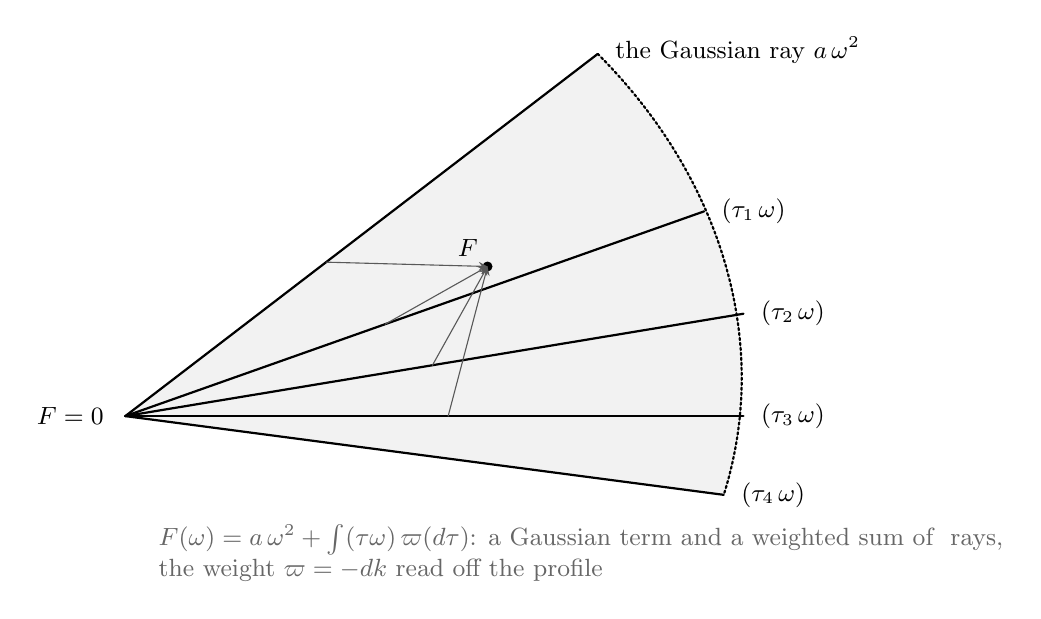
\begin{tikzpicture}[every node/.style={font=\small}, line cap=round, >=stealth]
\coordinate (O) at (0,0);
% the wedge
\fill[gray!10] (O) -- (6.0,4.6) .. controls (7.6,3.0) and (8.2,0.9) .. (7.6,-1.0) -- cycle;
\draw[thick] (O) -- (6.0,4.6);
\node[anchor=west] at (6.1,4.65) {the Gaussian ray $a\,\omega^2$};
% the Cin rays, one for each tau, along the far side
\foreach \x/\y/\lab in {7.35/2.6/{\tau_1}, 7.85/1.3/{\tau_2}, 7.85/0.0/{\tau_3}, 7.6/-1.0/{\tau_4}} {
  \draw[thick] (O) -- (\x,\y);
  \node[anchor=west] at (\x+0.1,\y) {$\Cin(\lab\,\omega)$};
}
\draw[thick, densely dotted] (6.0,4.6) .. controls (7.6,3.0) and (8.2,0.9) .. (7.6,-1.0);
\node[anchor=east] at (-0.15,0) {$F = 0$};
% a member as a superposition
\coordinate (F) at (4.6,1.9);
\fill (F) circle (1.8pt);
\node[anchor=south east] at (F) {$F$};
\draw[->, gray!70!black] (2.55,1.955) -- (F);
\draw[->, gray!70!black] (3.3,1.167) -- (F);
\draw[->, gray!70!black] (3.9,0.645) -- (F);
\draw[->, gray!70!black] (4.1,0.0) -- (F);
\node[anchor=north west, align=left, text=gray!80!black] at (0.3,-1.25)
  {$F(\omega) = a\,\omega^2 + \int \Cin(\tau\omega)\,\varpi(d\tau)$:
   a Gaussian term and a weighted sum of $\Cin$ rays,\\ the weight $\varpi = -dk$ read off the profile};
\end{tikzpicture}
\caption{The admissible cone, schematically. The exponents $F$ are the pairs $(a,k)$, a
Gaussian coefficient and a nonincreasing profile, and they form a convex cone
(Lemma~\ref{lem:admissible-cone}). Its extreme rays are the Gaussian ray, the member with no
jumps, and the $\Cin$ rays, one for each cutoff $\tau$, the exponents of the unit-step
profiles. Every member is a superposition of them in exactly one way, with the weights given
by the profile: a nonincreasing profile is a stack of unit steps, and $\varpi = -dk$ says how
much of each (Proposition~\ref{prop:choquet-cone}). The drawing shows that superposition and
nothing else; the cone has infinitely many dimensions, and where the named families and the
image of the bridge lie in it is the subject of Figure~\ref{fig:filtration} and of the chain
in \S\ref{sec:thorin}.}
\label{fig:admissible-cone}
\end{figure}


The proof has three parts. The domain condition on $\varpi$ is the two integrability
conditions of Lemma~\ref{lem:profile-integrability}, read on the tail measure through the
layer cake, which gives surjectivity. Injectivity is the uniqueness of the \Levy{} pair, with
two measure-theoretic steps that carry an equality of tails at almost every point to an
equality of measures. The extremality clauses are read at the profile, and the classification
of \emph{all} extreme rays is the one place the coordinates are used.

\begin{proof}
An admissible $F$ has, by Theorem~\ref{thm:main-characterization}, a pair $(a,k)$ of the form
\ref{eq:sd-profile}; a positive measure $\varpi$ on $(0,\infty)$ with
$k(x) = \varpi((x,\infty))$ almost everywhere exists by Lemma~\ref{lem:cin-rays}(2), and
\ref{eq:cone-superposition} is then the displayed representation. Conversely a pair
$(a,\varpi)$ in the stated domain gives back an admissible $F$: its profile is the tail
$k(x) = \varpi((x,\infty))$, nonnegative and nonincreasing, and the two integrability
conditions of Lemma~\ref{lem:profile-integrability} are the domain condition read through
Tonelli,
\[
  \int_0^1 x\,\varpi((x,\infty))\,dx = \int \tfrac12(\tau \wedge 1)^2\,\varpi(d\tau),
  \qquad
  \int_1^\infty \varpi((x,\infty))\,\frac{dx}{x} = \int \log_+\tau\,\varpi(d\tau),
\]
two more instances of the layer cake of Lemma~\ref{lem:cin-rays}(2), with the weights $x$ cut
off above $1$ and $x^{-1}$ cut off below $1$. Since
$\tfrac12(\tau\wedge1)^2 + \log_+\tau \le \tau^2 \wedge (1 + \log_+\tau)
 \le 2\bigl[\tfrac12(\tau\wedge1)^2 + \log_+\tau\bigr]$ for $\tau > 0$, the domain condition and
the two integrability conditions are the same condition. So the map is onto the cone, and the
domain is what the statement says.

That the superposition integral is finite at one $\omega \ne 0$ if and only if at all, and if
and only if the domain condition holds, follows. Sufficiency is the paragraph just given
together with Lemma~\ref{lem:quadratic-growth}, which makes an admissible exponent finite at
every frequency. For necessity it is enough to dominate $\tau^2 \wedge (1 + \log_+\tau)$ by a
multiple of $\Cin(\tau|\omega|)$ pointwise on $(0,\infty)$, and three regimes do that, using
only \emph{lower} bounds on $\Cin$. Below $\tau|\omega| = 1$ the expansion at the origin gives
$\Cin(z) \ge \tfrac{19}{96}z^2$, which dominates $\tau^2$ up to the constant
$|\omega|^{-2}$. Past a threshold the expansion at infinity gives
$\Cin(z) \ge \tfrac12(1 + \log z)$, which dominates $1 + \log_+\tau$ up to a constant once
$\tau$ is large enough that $\log(\tau|\omega|)$ is at least half of $\log\tau$. On the bounded
stretch between the two, monotonicity alone suffices:
$\Cin(\tau|\omega|) \ge \Cin(1) \ge \tfrac{19}{96}$ there, while $1 + \log_+\tau$ is bounded.
The map is linear in $(a,\varpi)$ by construction, both clauses being additivity of the
integral in the measure and positive homogeneity. It is injective because the pair of $F$ is
unique (Proposition~\ref{prop:fourier-toolbox}(3)): the pair determines $a$ and the \Levy{}
measure $k(x)x^{-1}dx$, hence $k$ up to a null set, hence the tails $\varpi((x,\infty))$ at
almost every $x > 0$. Two steps carry that to $\varpi$ itself. First, the exceptional set being
null, every interval $(x, x + \varepsilon)$ contains a point $y$ at which the two tails agree,
and $\varpi_1((x + \varepsilon,\infty)) \le \varpi_1((y,\infty)) = \varpi_2((y,\infty)) \le
\varpi_2((x,\infty))$; letting $\varepsilon$ decrease and using continuity of a measure along
the increasing sets $(x + \varepsilon, \infty)$ gives equality of the tails at \emph{every}
$x > 0$. Second, the tails at positive points are finite, by the domain condition, so for each
$\varepsilon > 0$ the restrictions of $\varpi_1$ and $\varpi_2$ to $(\varepsilon,\infty)$ are
finite measures agreeing on every half-line $(-\infty,t]$, since $\varpi((\varepsilon,t])$ is a
difference of two finite tails; two finite measures on $\RR$ agreeing on all such half-lines are
equal. Letting $\varepsilon$ decrease again, and using that $\varpi_1$ and $\varpi_2$ give no
mass to $(-\infty,0]$, gives $\varpi_1 = \varpi_2$. The detour through a finite restriction is
not avoidable by a direct $\pi$-system argument on the line: the Choquet measure of an unbounded
profile has infinite mass near the origin, so no exhausting sequence of finite-measure
half-lines exists before the restriction is made.

Extremality of the two named families is read at the profile, not through the coordinates. If
$\omega^2 = F_1 + F_2$ with both summands admissible, then $F_1 + F_2$ has pair $(1,0)$ by
uniqueness, so $k_1 + k_2$ vanishes almost everywhere on $(0,\infty)$, so each $k_i$ does, and
$F_i(\omega) = a_i\,\omega^2$ with $a_i \ge 0$: the Gaussian ray is extreme. If
$\Cin(\tau\,\cdot) = F_1 + F_2$, then uniqueness gives $a_1 = a_2 = 0$ and
$k_1 + k_2 = \mathbf 1_{(0,\tau)}$ almost everywhere; on the conull set inside $(0,\tau)$ where
that holds, each $k_i$ is nonincreasing, being a profile, and nondecreasing, being what is left
of a constant after subtracting a nonincreasing function, hence constant there, while above
$\tau$ both vanish by nonnegativity. So $k_i = c_i\,\mathbf 1_{(0,\tau)}$ almost everywhere and
$F_i = c_i\,\Cin(\tau\,\cdot)$ with $c_i \ge 0$: each $\Cin$ ray is extreme.

That there are no other extreme rays is where the coordinates are used, and where the
injectivity just proved is spent. Let $F$ be extreme with pair $(a,\varpi)$. If $\varpi = 0$
then $k$ vanishes almost everywhere and $F(\omega) = a\,\omega^2$. If $\varpi \ne 0$ then
$a = 0$: otherwise splitting $F$ as $a\,\omega^2$ plus the pure-jump part makes $a\,\omega^2$
equal to $c_1F$ for some $c_1$, and either $c_1 = 0$, forcing $a = 0$, or $F$ is a multiple of
$\omega^2$, which by uniqueness forces $\varpi = 0$. Now suppose some $s > 0$ has
$\varpi((0,s]) > 0$ and $\varpi((s,\infty)) > 0$. The restrictions of $\varpi$ to $(0,s]$ and to
$(s,\infty)$ split $F$ into two admissible exponents; extremality makes the first of them
$c_1F$; injectivity turns that into an equality of measures, the restriction of $\varpi$ to
$(0,s]$ against $c_1\varpi$; evaluating both sides on $(s,\infty)$ forces $c_1 = 0$, and then
$\varpi((0,s]) = 0$, a contradiction. So every $s$ has mass on at most one side. Put
$\tau := \inf\{s > 0 : \varpi((0,s]) > 0\}$, a set that is nonempty because $\varpi \ne 0$.
Then $\varpi((x,\infty)) = 0$ for $x > \tau$, by the defining property of the infimum together
with the hypothesis just established, hence also at $x = \tau$; and $\varpi((0,x]) = 0$ for
$0 < x < \tau$, by minimality. So $\varpi$ is carried by the single point $\tau$, which is
positive since otherwise $\varpi$ would be $0$, and $F = c\,\Cin(\tau\,\cdot)$ with
$c = \varpi(\{\tau\})$, finite because $\varpi((\tau/2,\infty))$ is. This is the map's own
picture: $(1,0) \mapsto \omega^2$, the Gaussian ray, and
$(0,\delta_\tau) \mapsto \Cin(\tau\,\cdot)$, whose profile is
$k(x) = \delta_\tau((x,\infty)) = \mathbf 1_{(0,\tau)}(x)$ and whose folded \Levy{} density is
therefore $x^{-1}\mathbf 1_{(0,\tau)}(x)$.
\end{proof}

The remark that follows compares the cone with that of the causal theory. The causal
article's cone is the cone of exponents of the
scale spaces on the temporal half-line, its ray off the curve is the \emph{drift}, the pure
delay, and its unit-step members are the \emph{Dickman rays}, whose kernels are the laws of
the Dickman subordinator (\sscite{caravenna2019dickman}). The Thorin subclass named in it is
the subcone of the profiles that are completely monotone, mixtures of exponentials, which
\S\ref{sec:corners} treats; the three named families are the subject of that section.

% blueprint rem:cone-shape, copied; this section's one relation-to-the-causal-theory remark
% (ADR-0003). The blueprint's chapter references are section references or, for the line
% paper's nodes, that paper's numbers; the causal article is named where the blueprint says
% "the causal cone" and "the causal remark".
\begin{remark}[what the cone looks like, and what changed]\label{rem:cone-shape}
In the log-displacement coordinate of Remark~\ref{rem:displacement-dictionary} the proposition
reads: every nonincreasing profile is a unique positive stack of unit steps, and every
admissible family is that stack plus one number $a$, a point \emph{off} the curve. The three
distinguished families of this paper are slices cut by different principles: the symmetric
stable family by dilation symmetry
(Corollary~\ref{cor:semigroup-case}), the \Matern{} family as the single-atom member of the
Thorin subclass (Theorem~\ref{thm:matern}), and the Student-t family as the image of the
causal Bessel corner under the bridge (Proposition~\ref{prop:student-t}). No member of the three
is an extreme ray of the cone, with one exception at an endpoint: the stable family closes at
$\alpha = 2$ on the Gaussian ray (Proposition~\ref{prop:stable-family}), which is extreme. All
three lie
in the Thorin subcone, each by the node that states it: the \Matern{} family as the one-atom
case of Proposition~\ref{prop:thorin-subclass}(2), the stable family by its Thorin density
(Proposition~\ref{prop:stable-family}), and the Student-t family by
Proposition~\ref{prop:student-t}(3), whose Thorin half is proved under the hypothesis that the
causal delay law is a generalized gamma convolution, a cited fact
(Remark~\ref{rem:student-ggc}).
The $\Cin$ rays are the paradigm of what lies outside it: profiles with a hard cutoff, whose
kernels carry derivative singularities at the displacements $\pm\tau, \pm2\tau, \dots$, echoes
of the step (Lemma~\ref{lem:cin-delay-equation}). Two things are new against the causal cone of
\sscite{fagerstrom2026hemigroup}. The Gaussian ray is an extreme ray of every subcone in the
chain $\IDs \supset \SDs \supset \GGCs$ --- the symmetric infinitely divisible laws, the
symmetric self-decomposable ones, and the symmetric Thorin subclass of
\S\ref{sec:thorin} --- being present in each with $k \equiv 0$, whereas the
corresponding causal ray, the drift, was the degenerate member. And the $\Cin$ rays, unlike
their causal counterparts, are not the image of anything under the bridge of
\S\ref{sec:bridge} (Proposition~\ref{prop:bridge-strictness}). The tail statement of the causal
article's cone remark holds here in a different shape but with the same conclusion: by
Proposition~\ref{prop:moments-tails}(2) a $\Cin$ kernel has tails of order
$e^{-|x|\log|x|/\tau}$, lighter than any exponential and heavier than any Gaussian; any
admissible kernel with a jump catalogue has tails at least that heavy, whatever its Gaussian
coefficient; and the only admissible kernels with Gaussian tails are the Gaussians themselves.
No truncation of the Gaussian is admissible.
\end{remark}

\subsection{The delay equation of the \texorpdfstring{$\Cin$}{Cin} kernels}\label{sec:delay-equation}

The kernel $p_\tau$ of a $\Cin$ ray, the density of the law with transform
$e^{-\Cin(\tau\omega)}$, has no closed form, and it satisfies a delay equation. A \emph{delay
equation} relates the derivative of a function at $x$ to the values of the function at a
fixed distance from $x$; the classical example is the equation
\[
  x\,\rho'(x) = -\rho(x - 1)
\]
of the Dickman function $\rho$ (\sscite{dickman1930frequency}; \sscite{tenenbaum2015introduction},
Chapter~III.5). It arose in number theory, where $\rho(u)$ is the limiting proportion of the
integers up to $n$ with no prime factor above $n^{1/u}$. Up to scale and a normalizing
constant it is also the density of the causal unit-step member, the Dickman subordinator of
\sscite{caravenna2019dickman}. The lemma of this subsection says that $p_\tau$ satisfies the
same equation with the average of the two neighbours $p_\tau(x \mp \tau)$ in place of the one
delayed value, because displacements come in both signs. The reason to want the equation is
what it says about the shape of the kernel. The derivative at $x$ is read off the values at
$x \pm \tau$, so a singularity at the origin reappears, smoothed, at $\pm\tau$, then at
$\pm2\tau$, and so on down the lattice $\tau\ZZ$. Figure~\ref{fig:cin-rays} shows these echoes
numerically and Remark~\ref{rem:cin-propagation} describes them. The description is not
proved here, and no result depends on it. The echoes are the signature of a hard cutoff in
the profile, and the smooth members of \S\ref{sec:corners} do not have them.

% shared with blueprint lem:cin-delay-equation
\begin{lemma}[the $\Cin$ kernels satisfy a delay equation]\label{lem:cin-delay-equation}
Let $p_\tau$ be the density of the symmetric law with exponent $\Cin(\tau\,\cdot)$ --- folded
profile $\mathbf 1_{(0,\tau)}$, two-sided \Levy{} density
$\tfrac12|x|^{-1}\mathbf 1_{(0,\tau)}(|x|)$, no Gaussian part --- and let $P_\tau$ be its
distribution function. Then, in the sense of distributions,
\[
  x\,p_\tau(x) = P_\tau(x) - \tfrac12\bigl[P_\tau(x-\tau) + P_\tau(x+\tau)\bigr],
  \qquad\text{equivalently}\qquad
  x\,p_\tau'(x) = -\tfrac12\bigl[p_\tau(x-\tau) + p_\tau(x+\tau)\bigr].
\]
\end{lemma}

The identity is asserted in the sense of distributions, which is what the transform argument
delivers; both sides are locally integrable, so it is also an almost-everywhere identity. Read
at the law rather than at the density the two displays are one statement, an identity between
two finite signed measures, and that is how the proof is organised; the passage back to the
density is a change of variables for the first display and one integration by parts for the
second.

\begin{proof}
Write $\mu$ for the law, $c(\omega) = \int\cos(\omega x)\,\mu(dx) = e^{-\Cin(\tau\omega)}$ for
its transform, and $\kappa_\tau$ for Lebesgue measure on $[0,\tau)$. Everything follows from one
identity between finite signed measures on $\RR$:
\begin{equation}\label{eq:cin-delay-measures}
  2\,x\,\mu(dx) \;=\; \nu - \nu_\tau ,
  \qquad \nu := \mu * \kappa_\tau, \quad
  \nu_\tau := \text{the image of $\nu$ under } x \mapsto x - \tau .
\end{equation}
By Tonelli, $\nu$ has Lebesgue density $x \mapsto \mu((x-\tau,x])$ and $\nu_\tau$ has density
$x \mapsto \mu((x,x+\tau])$; both are finite measures of total mass $\tau$. The left-hand side
is finite because $\mu$ has a finite first absolute moment: $\Cin(z) \le z^2/4$, so the exponent
of $\mu$ is quadratically flat, the truncation inequality of
Theorem~\ref{thm:increments-levy} gives $\mu\{|x| > R\} = O(R^{-2})$, and the layer cake
integrates that tail.

\emph{The transforms.} Since $\mu$ is symmetric, $\int x\,e^{-i\omega x}\mu(dx)$ has no real
part, the integrand's cosine half being odd, so it equals $-i\int x\sin(\omega x)\,\mu(dx)$. The
first absolute moment lets $c$ be differentiated under the integral sign, giving
$c'(\omega) = -\int x\sin(\omega x)\,\mu(dx)$; and differentiating $c = e^{-\Cin(\tau\cdot)}$ by
the chain rule gives $c'(\omega) = -\tau\,\Cin'(\tau\omega)\,c(\omega)$ with
$\Cin'(v) = (1-\cos v)/v$. The two readings of $c'$ are the elementary delay ODE
\begin{equation}\label{eq:cin-delay-ode}
  \omega\,c'(\omega) = -\,c(\omega)\,\bigl(1 - \cos\tau\omega\bigr),
\end{equation}
and together they give
$\int x\,e^{-i\omega x}\mu(dx) = -i\,\tau\,\Cin'(\tau\omega)\,c(\omega)$, which for
$\omega \ne 0$ is $-i\,(1-\cos\tau\omega)\,c(\omega)/\omega$. On the other side, the transform of
a convolution is the product, so
\[
  \hat\nu(\omega) = c(\omega)\int_0^\tau e^{-i\omega u}\,du
    = c(\omega)\,\frac{1 - e^{-i\omega\tau}}{i\omega},
  \qquad \hat\nu_\tau(\omega) = e^{i\omega\tau}\,\hat\nu(\omega),
\]
whence, for $\omega \ne 0$,
\[
  \hat\nu(\omega) - \hat\nu_\tau(\omega)
    = c(\omega)\,\frac{(1 - e^{-i\omega\tau})(1 - e^{i\omega\tau})}{i\omega}
    = c(\omega)\,\frac{2 - 2\cos\omega\tau}{i\omega}
    = -2i\,\frac{1 - \cos\omega\tau}{\omega}\,c(\omega),
\]
which is twice the transform of $x\,\mu(dx)$, that is, the transform of the left-hand side of \ref{eq:cin-delay-measures}; at $\omega = 0$ both
sides vanish, the left by symmetry and the right because $\nu$ and $\nu_\tau$ have equal mass.

\emph{Uniqueness.} Both sides of \ref{eq:cin-delay-measures} are signed, so
Proposition~\ref{prop:fourier-uniqueness} is applied after recombination: writing $x^{\pm}$
for the positive and negative parts of $x$, the two \emph{positive} finite measures
$2\,x^{+}\mu(dx) + \nu_\tau$ and $2\,x^{-}\mu(dx) + \nu$ have the same transform
by the display above, hence are equal, which is \ref{eq:cin-delay-measures}.

\emph{The two displays.} The first is \ref{eq:cin-delay-measures} read at Lebesgue densities.
With $\mu(dx) = p_\tau(x)\,dx$ the left-hand side has density $2x\,p_\tau(x)$ and the right-hand
side has density
\[
  \mu((x-\tau,x]) - \mu((x,x+\tau])
  = 2\Bigl(P_\tau(x) - \tfrac12\bigl[P_\tau(x-\tau) + P_\tau(x+\tau)\bigr]\Bigr),
\]
and two integrable functions with the same integral against every bounded measurable test
function agree almost everywhere --- it is enough to test against the sign of their difference.
The second display is \ref{eq:cin-delay-measures} paired with $\varphi'$ for a test function
$\varphi \in C_c^\infty$. Since $\int_0^\tau \varphi'(x+u)\,du = \varphi(x+\tau) - \varphi(x)$,
and likewise for $\nu_\tau$ with $x$ shifted, pairing gives
\[
  2\int x\,\varphi'(x)\,\mu(dx)
   = \int\bigl[\varphi(x+\tau) + \varphi(x-\tau)\bigr]\mu(dx) - 2\int \varphi\,d\mu ,
\]
that is $\int (x\varphi)'\,d\mu = \tfrac12\int[\varphi(\cdot+\tau) + \varphi(\cdot-\tau)]\,d\mu$;
and one integration by parts against the density turns that into the second display. One route
to the same identity convolves $\mu$ with the \emph{signed} weight
$y\,\nu_2(dy) = \tfrac12\sgn(y)\mathbf 1_{|y|<\tau}\,dy$, which is $\tfrac12$ of $\kappa_\tau$
minus its reflection. The computation above is that one with the two halves kept positive until
the subtraction at the end, so that no signed measure is convolved anywhere.
\end{proof}

\subsection{The behaviour at the origin}\label{sec:origin}

The last question of the section is what an admissible kernel looks like at the origin, the
point of zero displacement. A density is \emph{singular} at a point when it is
unbounded near it; the kernel of the exponent $\log(1+\omega^2)$, $e^{-|x|}/2$, is bounded with a
kink at the origin, the Gaussian is smooth there, and the $\Cin$ kernel of
Figure~\ref{fig:cin-rays} is unbounded. The answer, for every admissible kernel without a
Gaussian part, rests on two theorems of Sato on self-decomposable laws, and it depends on the profile
through one number, its value $c = k(0{+})$ at the origin: for $c < 1$ the density is
singular of the order $|x|^{c-1}K(|x|)$, for $c > 1$ it is continuous with
$\lceil c\rceil - 2$ derivatives, at $c = 1$ it is singular of the order of an integral of
$K$, and when $c$ is infinite the density is of class $C^\infty$. The factor $K$ is built from the profile, $K(y) = \exp\int_y^1 (c - k(u))\,du/u$. It is
slowly varying and at least $1$, and it measures how fast the profile approaches its value at
the origin. When the profile is constant near the origin, as for a $\Cin$ ray, $K$ is constant
there, the singularity below the threshold is the pure power and the one at the threshold is
a logarithm. In general $K$ is unbounded: the profile $\tfrac12 - 1/\log(1/x)$ near the origin
has $c = \tfrac12$ and a kernel of the order $|x|^{-1/2}\log(1/|x|)$. The intensity of small
displacements decides whether the kernel is bounded: a profile that starts
above $1$ produces enough small displacements to smooth the mass at the origin, and one that
starts below $1$ does not. The $\Cin$ rays start at exactly $1$.

\emph{The folding.} Sato's theorems are stated for a law on the line in terms of a
\emph{two-sided} profile $k_2$ on $\RR \setminus \{0\}$ and two constants,
$k_2(0{+}) + k_2(0{-})$ and $k_2(0{+}) - k_2(0{-})$, the second of which measures the
asymmetry of the law. This paper's profile is folded, as \S\ref{sec:exponents-recap} said:
the \Levy{} measure $k(x)x^{-1}dx$ lives on $(0,\infty)$ and counts both directions of a
displacement together, so a symmetric two-sided profile $k_2$ and its folding are related by
the factor $2$, $k = 2 k_2$ on $(0,\infty)$, and the sources' first constant is this paper's
$k(0{+})$ while the second is $0$. The lemma states the dictionary, so that the theorem can be
applied at the sources' own letter; the factor $2$ is the one place where a constant is easily
lost in carrying a statement from a source into this paper, and it is exactly what puts the
\Matern{} threshold at $\gamma = \tfrac12$ rather than at $\gamma = 1$ below.

% shared with blueprint lem:folding-translation
\begin{lemma}[the folding translation]\label{lem:folding-translation}
Let $(a,k)$ be a pair of the form \ref{eq:sd-profile} with $a = 0$, and suppose the folded
profile has a finite right limit $c := k(0{+})$ at the origin. Put $k_2(x) := \tfrac12 k(|x|)$
for $x \in \RR$. Then $k_2$ is a two-sided profile in the sense of the probabilistic sources:
it is nonnegative, nonincreasing on $(0,\infty)$, nondecreasing on $(-\infty,0)$, and
$\int_\RR (1 \wedge x^2)\,k_2(x)\,|x|^{-1}dx < \infty$. Its \Levy{} measure
$k_2(x)|x|^{-1}dx$ on $\RR \setminus \{0\}$ is the unfolding of $k(x)x^{-1}dx$:
\[
  \int_\RR \bigl(1 - \cos\omega x\bigr)\,\frac{k_2(x)}{|x|}\,dx
   = \int_0^\infty \bigl(1 - \cos\omega x\bigr)\,\frac{k(x)}{x}\,dx
   \qquad (\omega \in \RR),
\]
so the two forms specify the same symmetric law. Moreover $k_2(x) + k_2(-x) = k(x)$ for every
$x > 0$, and both one-sided limits at the origin exist, with
\[
  k_2(0{+}) = k_2(0{-}) = \tfrac12 c,
  \qquad\text{so that}\qquad
  k_2(0{+}) + k_2(0{-}) = c \quad\text{and}\quad k_2(0{+}) - k_2(0{-}) = 0 .
\]
\end{lemma}

The hypothesis that $c$ is finite is used only for the two limits; the structural conditions
and the exponent identity hold with no hypothesis at the origin.

Two further hypotheses of the sources are met by $k_2$ and are not visible in the lemma. The
singular and threshold regimes are stated for the driftless finite-variation form of the exponent,
which asks $\int_{|x|<1}k_2(x)\,dx < \infty$ and leaves no first-order term: with $c$ finite,
$k_2 \le \tfrac12c$ on each side of the origin by monotonicity, so that integral is at most $c$;
the drift vanishes because the law is specified through its cosine transform; and there is no
Gaussian part because $a = 0$. And the sources normalise a profile to the version left-continuous
on $(0,\infty)$ and right-continuous on $(-\infty,0)$, which $k_2$ need not be. Passing to that
modification changes $k_2$ on a countable set only, and hence changes neither the \Levy{} measure
$k_2(x)|x|^{-1}dx$, nor the exponent, nor the law, nor the two one-sided limits at the origin, nor
the functions $K$ and $L$ below, which are integrals of $k_2$. So the theorems apply to the
modification and conclude about the same law with the same comparison functions.

\begin{proof}
The three structural conditions are the corresponding conditions on $k$ read through
$x \mapsto |x|$: nonnegativity is immediate, and for $x \le y < 0$ one has $|x| \ge |y| > 0$, so
$k_2(x) \le k_2(y)$ because $k$ is nonincreasing on $(0,\infty)$. For the two integrals, note
first that the map $x \mapsto -x$ preserves Lebesgue measure and that both integrands below are
even, $\cos$ being even and $k_2$ being a function of $|x|$; so each integral over $\RR$ is
twice the corresponding integral over $(0,\infty)$, where $k_2 = \tfrac12 k$. The two factors
$2$ cancel, which gives the exponent identity, and the same computation turns
$\int_\RR (1 \wedge x^2)k_2(x)|x|^{-1}dx$ into $\int_0^\infty (1 \wedge x^2)k(x)x^{-1}dx$, which
is finite: on $(0,1)$ it is $\int_0^1 x\,k(x)\,dx$ and on $(1,\infty)$ it is
$\int_1^\infty k(x)x^{-1}dx$, the two conditions of Lemma~\ref{lem:profile-integrability}.

The pointwise identity is $k_2(x) + k_2(-x) = \tfrac12 k(x) + \tfrac12 k(x)$ for $x > 0$. For the
limits, $k_2$ agrees with $\tfrac12 k$ on $(0,\infty)$, so its right limit is $\tfrac12 c$; and
$k_2(x) = \tfrac12 k(-x)$ on $(-\infty,0)$, where $x \mapsto -x$ carries the left neighbourhood
filter at the origin to the right one, so its left limit is $\tfrac12 c$ as well. The sum and
the difference follow.
\end{proof}

\emph{The cited fact.} The three regimes are two theorems of Sato: the smooth regime is
\sscite{sato1999levy}, Theorem~28.4, p.~191, and the singular regime and the threshold are
Theorem~53.8, pp.~410--411, formulas (53.28) and (53.30) there, all stated for a
self-decomposable law on the line with no Gaussian part in terms of its two-sided profile and
the two constants above. This is the one fact of this section that is cited rather than
proved (\S\ref{sec:machine-checked}). What the proposition takes from the theorems is the
\emph{order} of the singularity, an unbounded representative below and at the threshold and
a continuous one above it, and not the constant in Sato's formula. It claims nothing when
$k(0{+}) = \infty$, which is the case for the stable profiles and for every completely
monotone profile with an unbounded Thorin measure; that case is
Corollary~\ref{cor:origin-smooth} at the end of this subsection, on a further clause of the same
theorem.

The order does need the constant in Sato's formula to be nonzero, since $f \sim Ag$ gives
$f \asymp g$ only for $A \ne 0$, and the folding is what makes it so. Below the threshold the
constant is $\kappa\sin(k_2(0{+})\pi)/\bigl(\Gamma(c)\sin(c\pi)\bigr)$ with $\kappa > 0$ the
exponential-integral expression of the source's (53.27), and $k_2(0{+}) = c/2$ turns the first
factor into $\sin(c\pi/2)/\sin(c\pi) = 1/\bigl(2\cos(c\pi/2)\bigr) > 0$ for $0 < c < 1$; at the
threshold it is $(\kappa/\pi)\cos(c'\pi/2)$ with $c' = 0$, hence $\kappa/\pi$. The symmetry is
therefore load-bearing twice, once for the antisymmetric constant and once for the nonvanishing.

% The proof below is the blueprint's of 2026-09-19 (R171) minus its two sentences on what is
% machine-checked (the author's decision D5; section 1.1 owns that account).
% shared with blueprint prop:cin-origin-singularity
\begin{proposition}[the behaviour of an admissible kernel at the origin]
\label{prop:cin-origin-singularity}
Let $F$ be admissible with Gaussian coefficient $0$ and folded profile $k$, let $\phi_1$ be its
kernel at canonical scale $1$, and suppose the right limit $c := k(0{+})$ is positive, so that
$c \in (0,\infty]$. The three regimes below
are stated for finite $c$, and nothing is claimed when $c = \infty$. For $0 < y < 1$ set
\[
  K(y) := \exp\Bigl[\int_y^1 \bigl(c - k(u)\bigr)\,\frac{du}{u}\Bigr],
  \qquad
  L(y) := \int_y^1 K(z)\,\frac{dz}{z},
\]
both integrals being convergent; $K \ge 1$, since $k$ is nonincreasing with right limit $c$. Then,
near the origin: if $c < 1$, $\phi_1$ is unbounded with $\phi_1(x) \asymp |x|^{c-1}K(|x|)$; if
$N < c \le N+1$ for an integer $N \ge 1$, $\phi_1$ extends continuously and has $N-1$ derivatives;
and if $c = 1$, $\phi_1$ is unbounded with $\phi_1(x) \asymp L(|x|)$. Every $\Cin$ ray has $c = 1$
with $K$ constant near the origin, so its kernel is logarithmically singular there.
\end{proposition}

None of the three regimes is empty: the threshold is met by the $\Cin$ rays, the singular
regime by the profile $c\,\mathbf 1_{(0,\tau)}$ with $c < 1$, and the smooth one by the
\Matern{} profile of \S\ref{sec:corners} at $\gamma = 1$, where $c = 2$ and the kernel is the
Laplace kernel, continuous with a kink.

\begin{proof}
The three regimes are the cited interface, and what has to be said here is how the source's
statement becomes this one. The sources state the behaviour at the origin of a self-decomposable
law with no Gaussian part in terms of its \emph{two-sided} profile $k_2$ on $\RR \setminus \{0\}$
and the two constants $k_2(0{+}) + k_2(0{-})$ and $k_2(0{+}) - k_2(0{-})$: the first is their
$c$, the second their antisymmetric constant. By Lemma~\ref{lem:folding-translation} the law in
question is theirs. Its two-sided datum is $k_2(x) = \tfrac12 k(|x|)$, which is a profile of the
kind the sources require; its exponent is the folded exponent, so the two descriptions specify
the same law; the first constant is $k(0{+}) = c$; and the second vanishes, the law being
symmetric. The three hypotheses of the sources that the dictionary does not display --- finite
variation near the origin, no drift and no Gaussian part, and the one-sided continuity of the
profile --- are met for the reasons given after the lemma. Reading the three regimes through that
dictionary gives the three statements
displayed above, with $k_2(u) + k_2(-u)$ becoming $k(u)$ in the integrand of $K$, which is the
factor both singular clauses carry, and the passage from the source's asymptotic to the two-sided
comparison uses the nonvanishing of the source's constant, computed above. The regimes themselves
are cited, and the order of the singularity is all that is claimed of them.

The last sentence is this paper's own. The $\Cin$ ray of step $\tau$ has profile
$\mathbf 1_{(0,\tau)}$ (Lemma~\ref{lem:cin-rays}(1)), whose right limit at the origin is $1$, so
$c = 1$ and the threshold regime applies; and on $(0,\tau)$ the integrand $(1 - k(u))u^{-1}$ of
$K$ vanishes, which is the constancy of an indicator on its own interval. So $K$ is constant on $(0,\min(\tau,1))$, with the value
$\max(1,1/\tau)$: for $\tau \ge 1$ nothing is integrated, and for $\tau < 1$ the window $(\tau,1)$
contributes $\int_\tau^1 u^{-1}du = \log(1/\tau)$. Hence $L$ is a constant multiple of
$\log(1/|x|)$ plus a constant near the origin --- $L(x) = \log(1/|x|)$ when $\tau \ge 1$ and
$L(x) = \tau^{-1}\log(\tau/|x|) + \tau^{-1} - 1$ when $\tau < 1$ --- and in both cases the
logarithmic order is all the statement claims.
\end{proof}

% blueprint rem:cin-propagation, copied
\begin{remark}[the singularity propagates outward]\label{rem:cin-propagation}
For a $\Cin$ ray of step $\tau$ the delay equation of Lemma~\ref{lem:cin-delay-equation}
carries the singularity outward along the lattice $\tau\ZZ$, one order of smoothness gained at
each step: the derivative of the kernel inherits a logarithmic singularity at $\pm\tau$, so the
kernel itself is continuous there with a kink of order $|x \mp \tau|\log|x \mp \tau|$, and so
on to $\pm2\tau$ and beyond. This is a description of the shape of the kernel and not a claim
of the proposition: the induction it summarises is not carried out here, and no result depends
on it.
\end{remark}

The $\Cin$ kernels are therefore logarithmically singular at the origin. So is one member of
the \Matern{} family of \S\ref{sec:corners}. That family consists of the \emph{variance-gamma}
laws, the laws of a Brownian motion run for a Gamma-distributed time
(\sscite{madan1990variance}). At the index $\gamma = \tfrac12$ its kernel is a multiple of
$K_0(|x|)$, the modified Bessel function of the second kind, which has a logarithmic
singularity at the origin and sits at the same threshold. Both are instances of a single
boundary in the cone, and where it falls is decided by the profile alone. The corollary says
that an admissible kernel with no Gaussian part, and with $k(0{+})$ finite and positive, is
bounded at the origin exactly when the profile starts above $1$. It then reads the condition
off for the named members. For the \Matern{} family it uses the profile
$2\gamma e^{-x/\theta}$, which is computed in \S\ref{sec:corners}
(Proposition~\ref{prop:matern-exponent}(1)) by an elementary integral that uses nothing of this
section, so the reference ahead is not circular.

% shared with blueprint cor:origin-boundedness
\begin{corollary}[the boundedness threshold]\label{cor:origin-boundedness}
Let $F$ be admissible with Gaussian coefficient $0$ and folded profile $k$, let $\phi_1$ be its
kernel at canonical scale $1$, and suppose $c := k(0{+})$ is finite and positive.
\begin{enumerate}
\item \emph{(The threshold.)} If $c > 1$, then $\phi_1$ has a representative continuous on the
whole line. If $c \le 1$, then for every representative $p$ of $\phi_1$, every $\delta > 0$ and
every $M$ there is an $x$ with $0 < |x| < \delta$ and $p(x) > M$; no representative of $\phi_1$
is bounded near the origin. So $\phi_1$ is bounded at the origin exactly when $c > 1$.
\item \emph{(The named members.)} Every $\Cin$ ray has $c = 1$ and sits at the threshold. The
\Matern{} member of index $\gamma$ and range $\theta$ has $c = 2\gamma$, so its kernel is
bounded at the origin exactly for $\gamma > \tfrac12$, and at $\gamma = \tfrac12$ it sits at the
threshold.
\end{enumerate}
\end{corollary}

Clause (2) is the boundary that the closed form of Proposition~\ref{prop:matern-density}
shows from the other side: the closed form is a \Matern{} covariance function only for
$\gamma > \tfrac12$, and is the Bessel $K_0$ at $\gamma = \tfrac12$. The corollary claims the
threshold and not the rate of the divergence there, which for this member is logarithmic and
is the cited Bessel asymptotic rather than anything proved here, and it says nothing in
dimension greater than one.

\begin{proof}
Both halves of clause (1) come from Proposition~\ref{prop:cin-origin-singularity}. If $c > 1$, choose the
integer $N \ge 1$ with $N < c \le N+1$ --- which exists for every finite $c > 1$, namely
$N = \lceil c\rceil - 1$ --- and the smooth regime gives a representative of $\phi_1$ that is
$C^{N-1}$ on the whole line, in particular continuous. Below the threshold and at it, both
comparison functions are handled by one bound on the slowly varying factor: $k$ is nonincreasing
on $(0,\infty)$ with right limit $c$, so $k \le c$ there, the integrand $(c-k(u))u^{-1}$ of $K$ is
nonnegative, and $K \ge 1$ on $(0,1)$. If $c < 1$ the singular regime gives a
representative $p_0$ and constants $c_1 > 0$, $\delta_0 > 0$ with
$p_0(x) \ge c_1|x|^{c-1}K(|x|) \ge c_1|x|^{c-1}$ for $0 < |x| < \delta_0$; if $c = 1$ the
threshold regime gives the same with $c_1 L(|x|)$ in place of $c_1|x|^{c-1}K(|x|)$, and
$L(x) \ge \int_{|x|}^1 z^{-1}dz = \log(1/|x|)$ by the same bound. In both cases
the lower bound tends to $+\infty$ as $x \to 0$.

That carries to every representative, and not only to $p_0$, by comparing measures rather than
functions. Suppose some representative $p$ satisfied $p \le M$ on the punctured
$\delta$-neighbourhood of the origin, and let $0 < \varepsilon \le \min(\delta,\delta_0)$. On
$(0,\varepsilon)$ the regime's lower bound is at least its value at $\varepsilon$, both
$|x|^{c-1}$ and $L$ being nonincreasing in $|x|$: below the threshold
$p_0 \ge c_1\varepsilon^{c-1}$ there, and at it $p_0 \ge c_1\log(1/\varepsilon)$. So
$\phi_1\bigl((0,\varepsilon)\bigr) \ge c_1\varepsilon^{c-1}\cdot\varepsilon$ in the first case
and $\ge c_1\log(1/\varepsilon)\cdot\varepsilon$ in the second, while the assumed bound on $p$
gives $\phi_1\bigl((0,\varepsilon)\bigr) \le M\varepsilon$. Dividing by $\varepsilon$ leaves
$c_1\varepsilon^{c-1} \le M$, respectively $c_1\log(1/\varepsilon) \le M$, and both left-hand
sides tend to $+\infty$ as $\varepsilon$ decreases. Choosing $\varepsilon$ small enough
contradicts the assumption. Neither step needs $p$ to be measurable: a density integrates over a
Borel set whatever representative names it, and the two bounds are bounds on that integral.

Clause (2) is the profile computation in each case. The $\Cin$ ray of step $\tau$ has profile
$\mathbf 1_{(0,\tau)}$, whose right limit at the origin is $1$ (Lemma~\ref{lem:cin-rays}(1)); the
\Matern{} profile at range $\theta$ is $2\gamma e^{-x/\theta}$ (Proposition~\ref{prop:matern-exponent}(1)),
whose right limit is $2\gamma$. Reading $c = 2\gamma$ through clause (1) puts the threshold at
$\gamma = \tfrac12$.
\end{proof}

The corollary leaves one case open, and it is the case of two of the three families of
\S\ref{sec:corners}: a profile that is unbounded at the origin, $k(0{+}) = \infty$. There the
same theorem of Sato on the smooth regime has a clause of its own --- if the two-sided constant is
infinite the law has a $C^\infty$ density (\sscite{sato1999levy}, Theorem~28.4, p.~191, clause
(ii)) --- and it settles the case in the other direction: an unbounded profile produces so many
small displacements that the kernel is not merely bounded at the origin but smooth there.

% shared with blueprint cor:origin-smooth
\begin{corollary}[an unbounded profile makes the kernel smooth]\label{cor:origin-smooth}
Let $F$ be admissible with Gaussian coefficient $0$ and folded profile $k$, and let $\phi_1$ be
its kernel at canonical scale $1$. If $k(0{+}) = \infty$, then $\phi_1$ has a representative of
class $C^\infty$ on $\RR$; in particular that representative is bounded on every bounded set, so
$\phi_1$ is bounded at the origin. The symmetric stable members of index $0 < \alpha < 2$ are of
this kind: their folded profile is a positive multiple of $x^{-\alpha}$
(Proposition~\ref{prop:stable-family}), whose right limit at the origin is $+\infty$.
\end{corollary}

With the Gaussian coefficient $0$ and $F \not\equiv 0$ the value $c = k(0{+})$ lies in
$(0,\infty]$, a nonincreasing profile with $k(0{+}) = 0$ vanishing identically. The two
corollaries therefore cover the whole range, and together they say one thing: \emph{an admissible
kernel with no Gaussian part is bounded at the origin exactly when its profile starts above $1$.}
What is claimed of the smooth case is the smoothness and nothing else --- no rate, no bound on
the density or its derivatives. The Student-t members have an unbounded profile as well, but this
paper does not prove it: what it has of that family's profile is the Gaussian mixture
\ref{eq:bridge-profile} of a causal catalogue it does not compute. Nothing is lost, since the
Student-t kernel is bounded at the origin by its own explicit density
(Proposition~\ref{prop:student-t}(1)).

\begin{proof}
The cited theorem is stated for a self-decomposable law on $\RR$ with no Gaussian part, presented
through a two-sided profile $k_2$ --- nonnegative, nonincreasing on $(0,\infty)$ and
nondecreasing on $(-\infty,0)$ --- and reads its conclusion off the constant
$c = k_2(0{+}) + k_2(0{-})$; at $c = \infty$ that conclusion is a $C^\infty$ density on the line.
That presentation is itself the hypothesis: the source says of it that it is the general form of
a purely non-Gaussian self-decomposable law on $\RR$, so exhibiting a law in it is exhibiting it
as one.
Put $k_2(x) := \tfrac12 k(|x|)$. The structural conditions and the exponent identity are the
first two paragraphs of the proof of Lemma~\ref{lem:folding-translation}, which read only the
monotonicity of $k$ and the two integrability conditions of
Lemma~\ref{lem:profile-integrability}: that lemma's hypothesis that $k(0{+})$ is finite is used
for its two one-sided limits alone, and is not available here. So $k_2$ is a two-sided profile of
the required kind, and its \Levy{} measure $k_2(x)|x|^{-1}dx$ specifies the same symmetric law as
the pair $(0,k)$, whose kernel at canonical scale $1$ is $\phi_1$. Both one-sided limits of $k_2$
at the origin are $+\infty$: on $(0,\infty)$ it is $\tfrac12k$, whose right limit is $+\infty$ by
hypothesis, and on $(-\infty,0)$ it is $x \mapsto \tfrac12k(-x)$, where $x \mapsto -x$ carries the
left neighbourhood filter at the origin to the right one. So the source's constant is $c = \infty$
and its clause applies. The one hypothesis the dictionary does not display is the source's
normalisation of a $k$-function to its one-sided-continuous version, discussed after
Lemma~\ref{lem:folding-translation}: passing to that modification changes $k_2$ on a countable set,
hence changes neither the \Levy{} measure nor the exponent nor the law, and leaves both one-sided
limits infinite.

The two consequences are elementary. A function of class $C^\infty$ on $\RR$ is continuous, hence
bounded on every compact set, so the representative the theorem produces is bounded on a
neighbourhood of the origin. And the symmetric stable member of index $\alpha$ has folded profile
$C_\alpha^{-1}x^{-\alpha}$ with $C_\alpha \in (0,\infty)$
(Proposition~\ref{prop:stable-family}), which tends to $+\infty$ as $x$ decreases to $0$.
\end{proof}
